\subsection{Memory}

These charts represent the memory usage of clients and servers during ephemeral and persistent experiments.

During persistent and ephemeral experiments, it’s possible to observe that \gls{udp} and \gls{tcp} had the lowest memory usage. However, \gls{tcp}+\gls{tls} was more than double. That can be explained by \gls{tls}’ data encryption overhead, which demands a bit more memory usage.

QUIC uses around double memory when compared to \gls{tcp}+\gls{tls} experiments. Nothing special since it’s expected to have more memory usage as a tradeoff for efficiency on unreliable networks. Nonetheless, on ephemeral experiments it had an interesting behaviour. On smaller data sizes it uses a ton of memory, around 10 times \gls{tcp}+\gls{tls}’, while only using half on the largest data size. This happens during ephemeral experimentations only because we are constantly creating and deleting clients, therefore Go’s garbage collector is unable to quickly clean unused clients. On smaller data sizes, the rate of client creation is higher because the requests end faster, in contrast to big data sizes, which require more time to complete requests, allowing Go’s garbage collector more time to do its job.

\clearpage

\begin{figure}[h!]
    \centering
    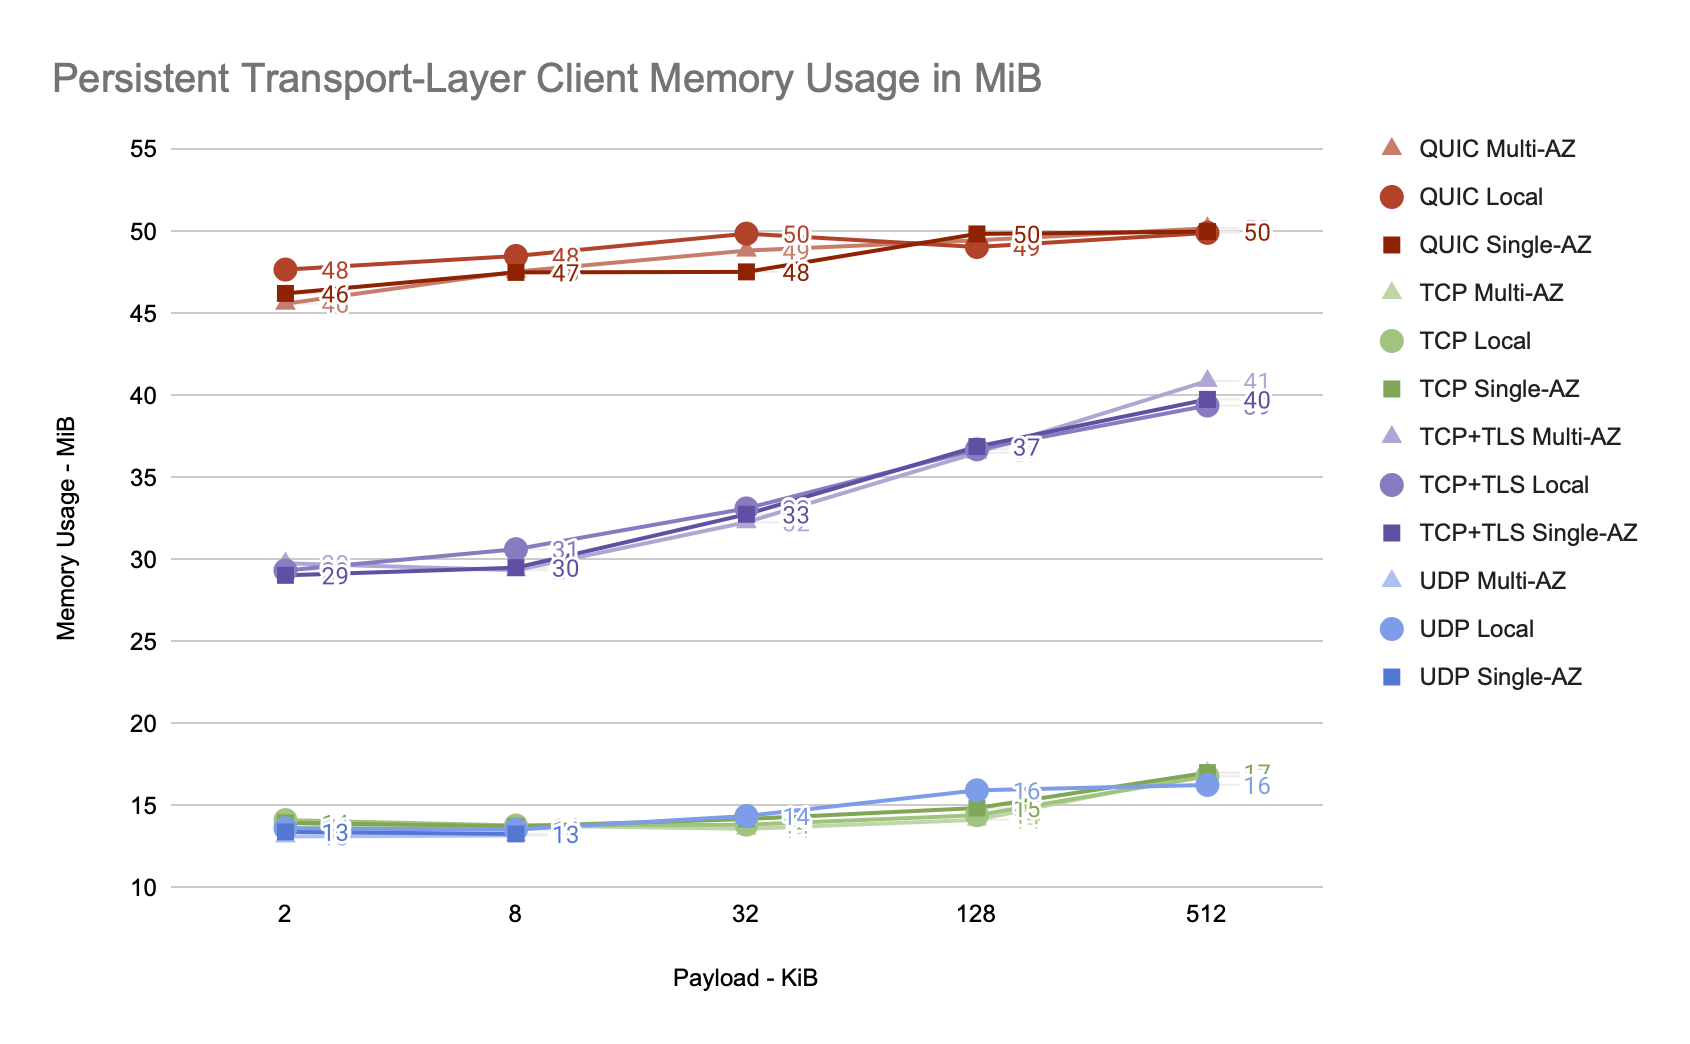
\includegraphics[width=\linewidth]{figures/charts/Persistent Transport-Layer Client Memory Usage in MiB.png}
    \caption{Persistent Transport-Layer Client Memory Usage in MiB}
    \label{fig:persistent_client_transport_memory}
\end{figure}

\begin{figure}[h!]
    \centering
    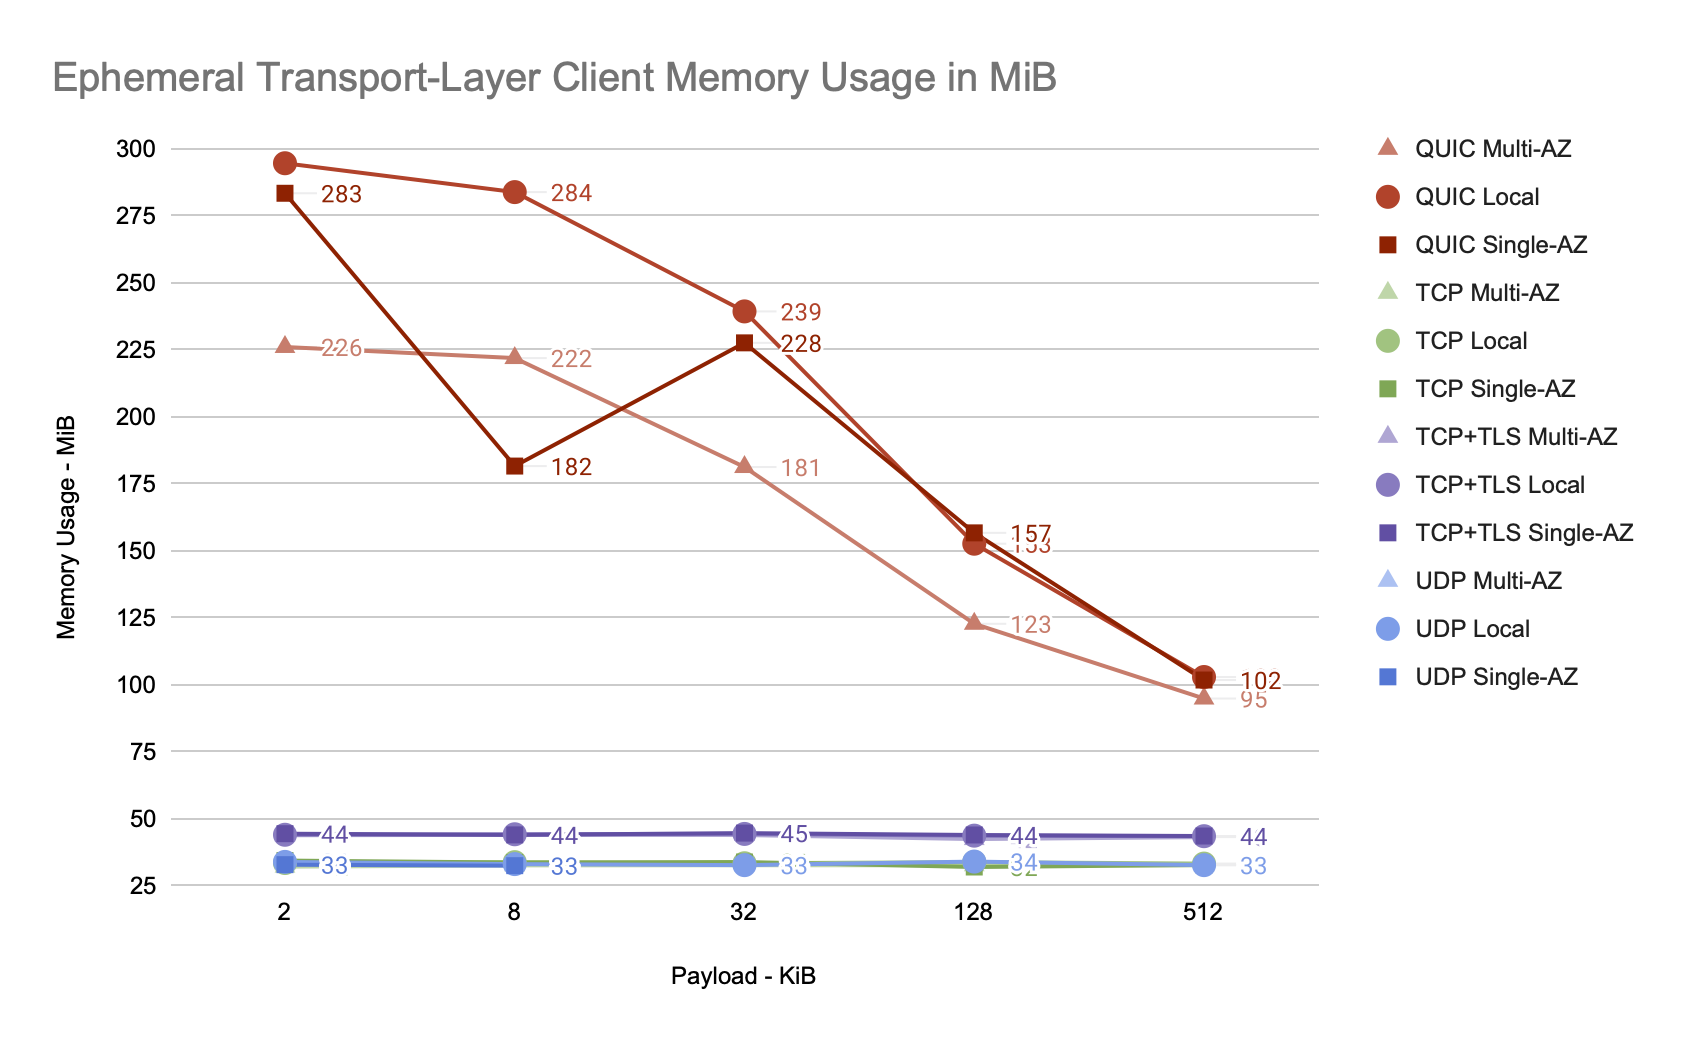
\includegraphics[width=\linewidth]{figures/charts/Ephemeral Transport-Layer Client Memory Usage in MiB.png}
    \caption{Ephemeral Transport-Layer Client Memory Usage in MiB}
    \label{fig:ephemeral_client_transport_memory}
\end{figure}

\begin{figure}[h!]
    \centering
    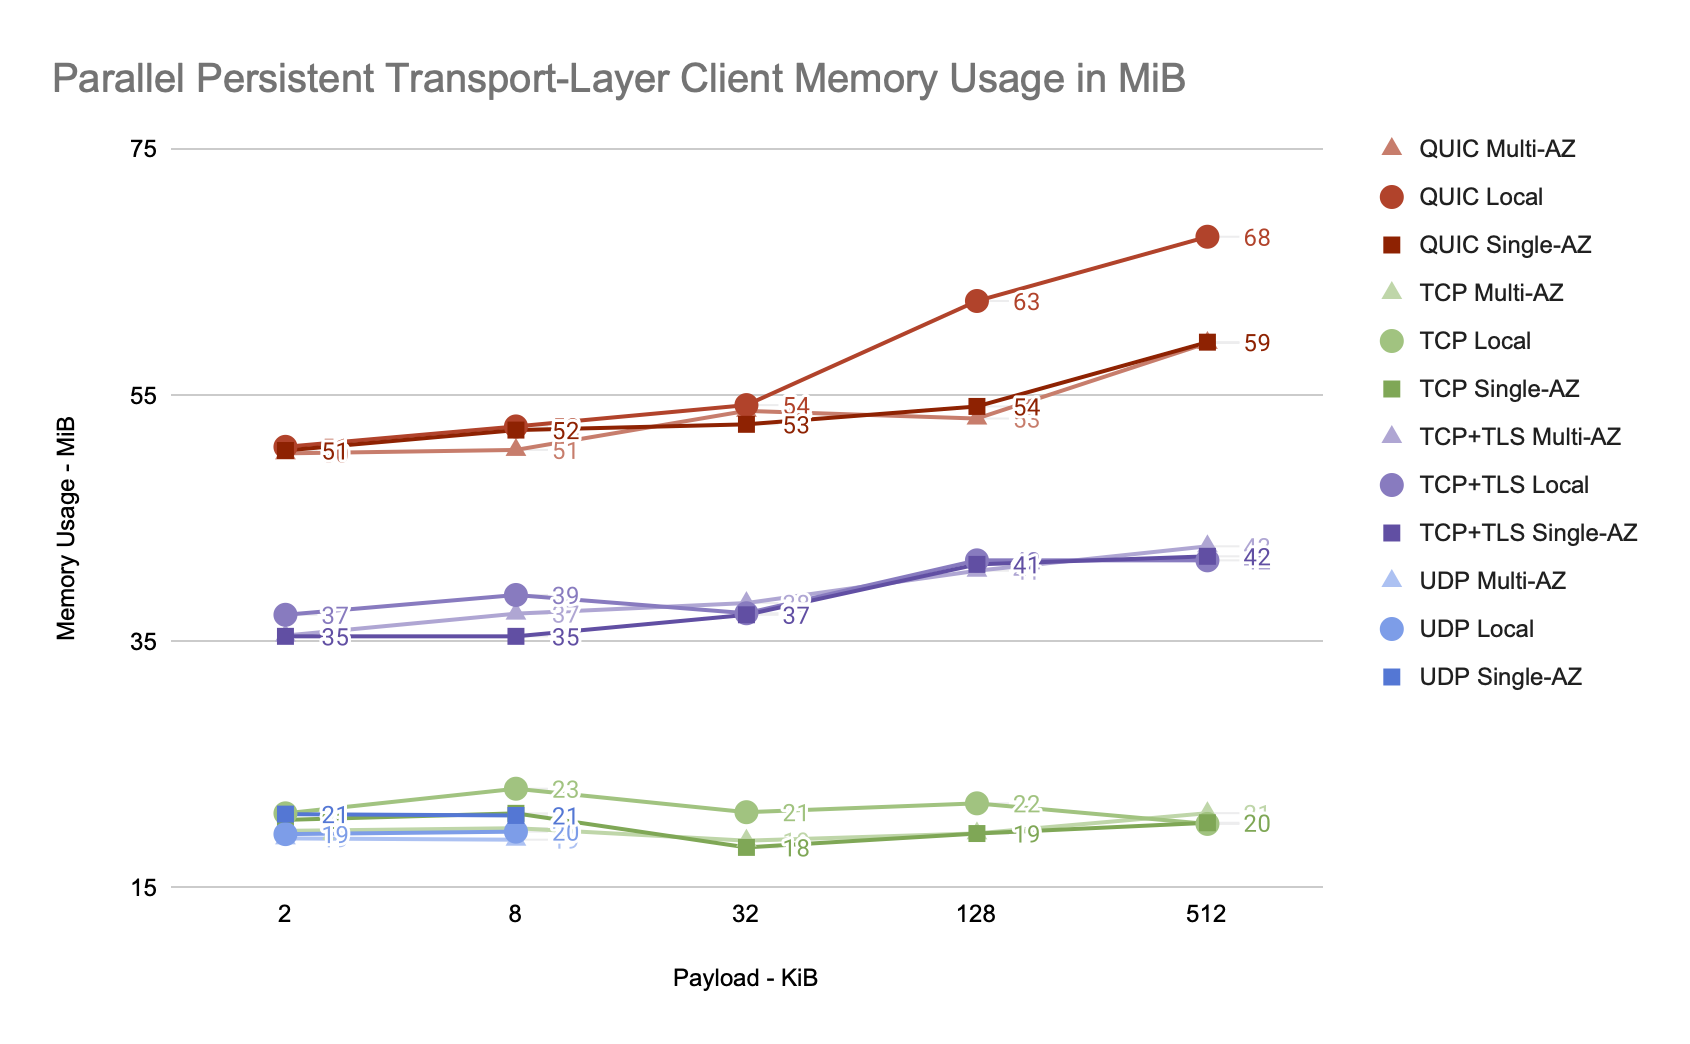
\includegraphics[width=\linewidth]{figures/charts/Parallel Persistent Transport-Layer Client Memory Usage in MiB.png}
    \caption{Parallel Persistent Transport-Layer Client Memory Usage in MiB}
    \label{fig:parallel_client_transport_memory}
\end{figure}

\begin{figure}[h!]
    \centering
    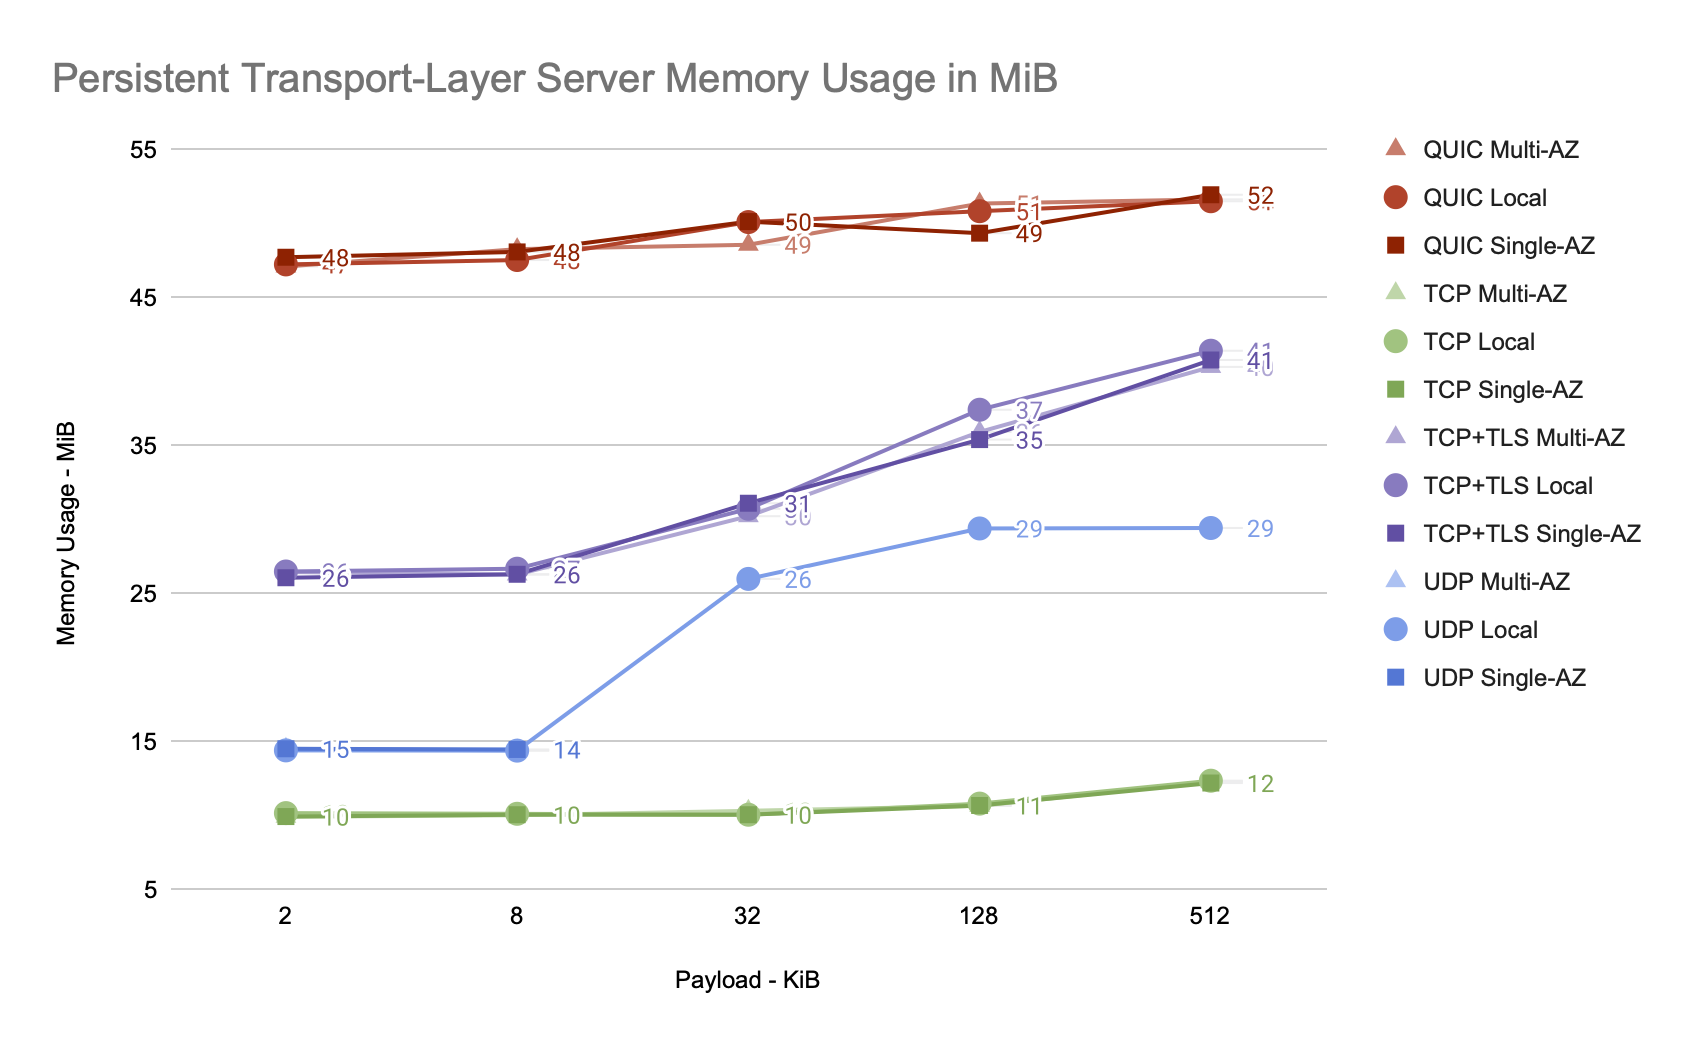
\includegraphics[width=\linewidth]{figures/charts/Persistent Transport-Layer Server Memory Usage in MiB.png}
    \caption{Persistent Transport-Layer Server Memory Usage in MiB}
    \label{fig:persistent_server_transport_memory}
\end{figure}

\begin{figure}[h!]
    \centering
    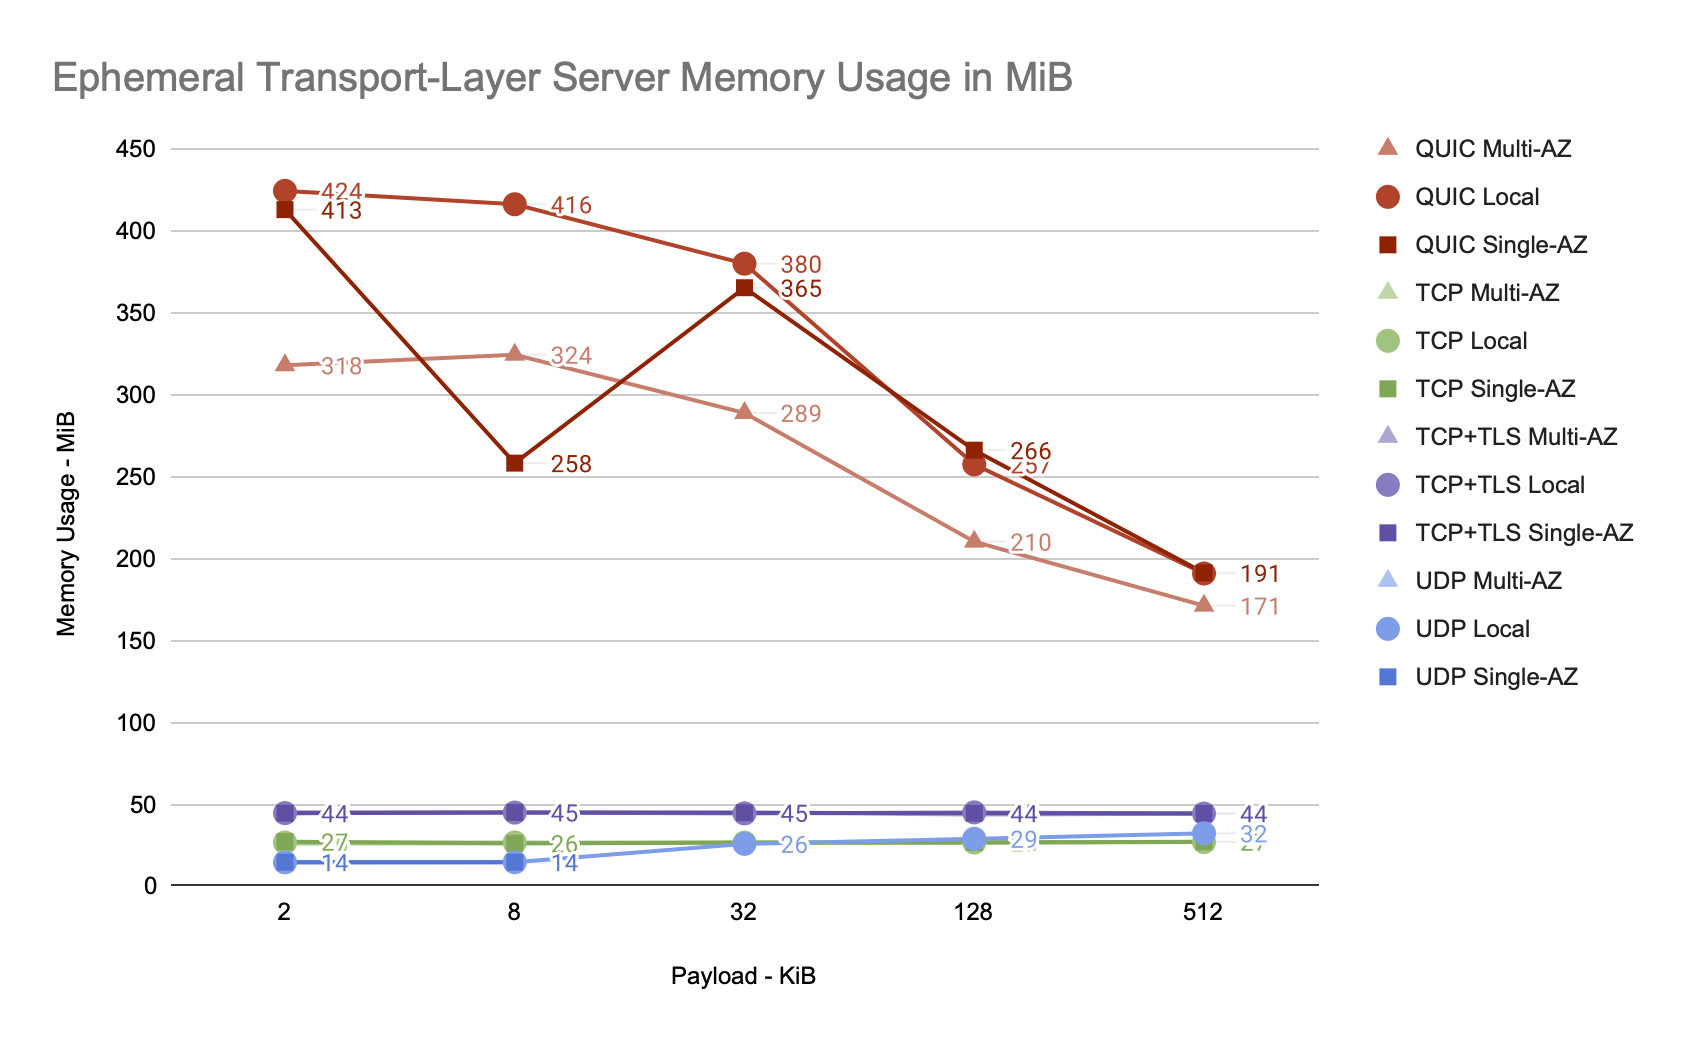
\includegraphics[width=\linewidth]{figures/charts/Ephemeral Transport-Layer Server Memory Usage in MiB.png}
    \caption{Ephemeral Transport-Layer Server Memory Usage in MiB}
    \label{fig:ephemeral_server_transport_memory}
\end{figure}

\begin{figure}[h!]
    \centering
    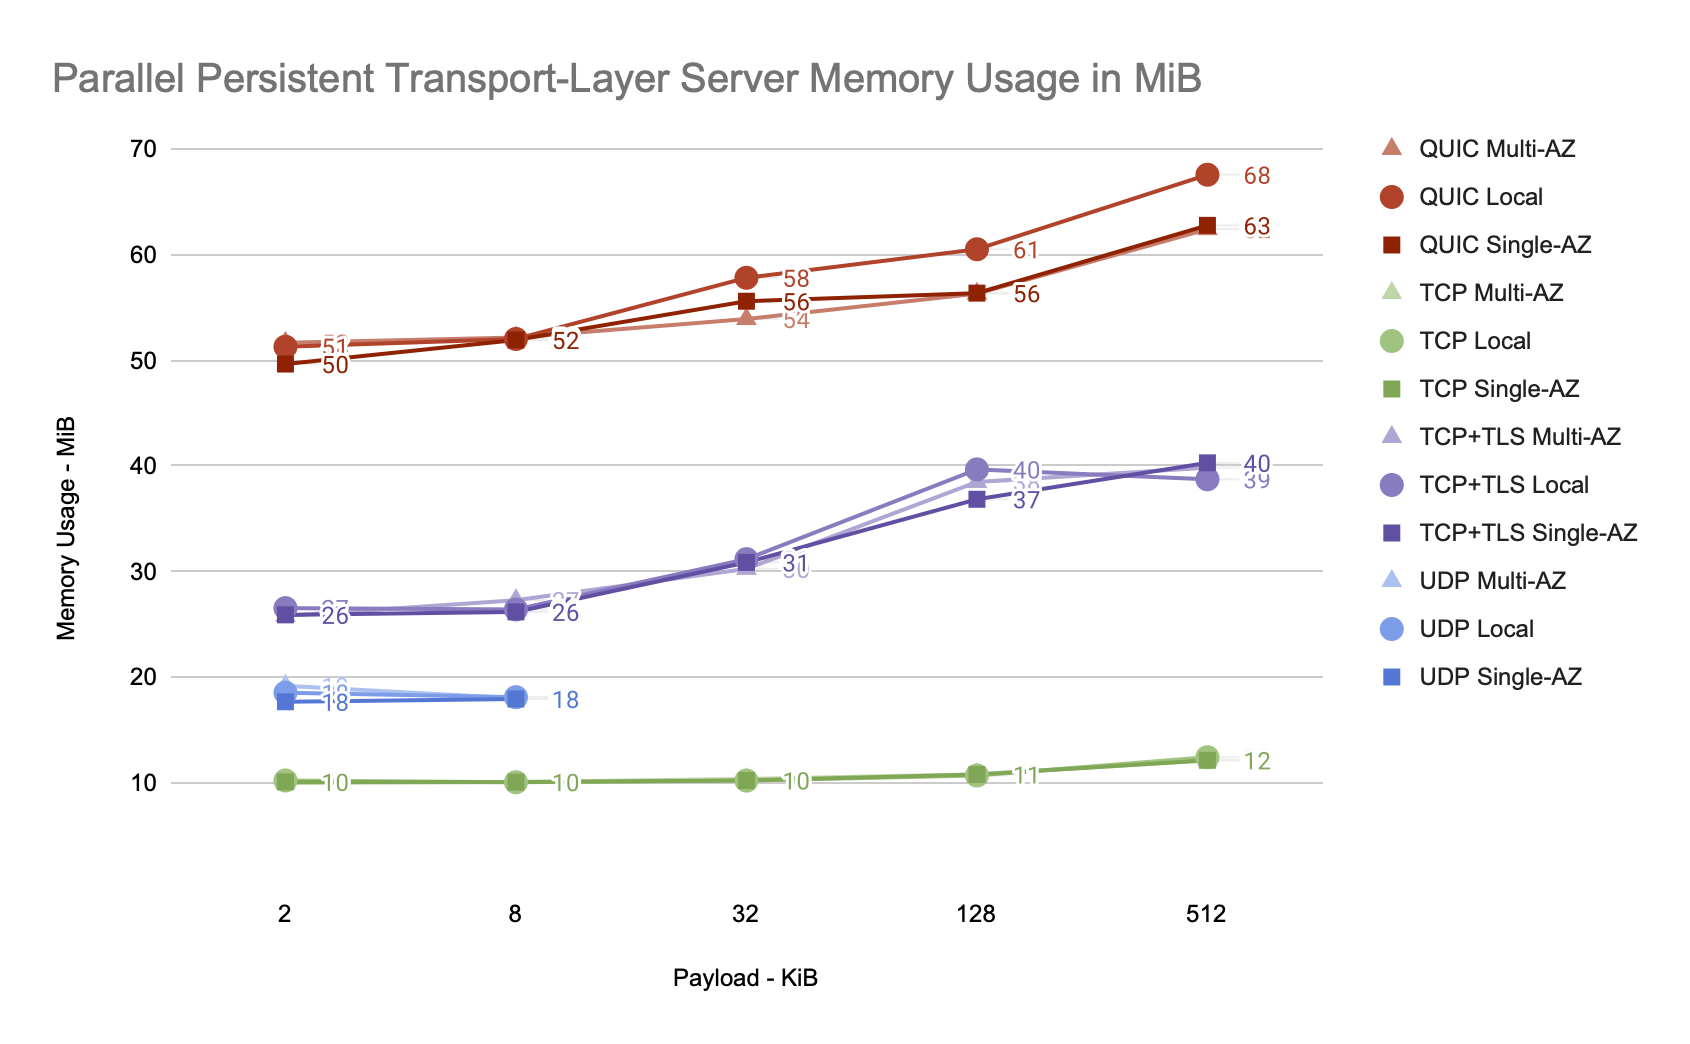
\includegraphics[width=\linewidth]{figures/charts/Parallel Persistent Transport-Layer Server Memory Usage in MiB.png}
    \caption{Parallel Persistent Transport-Layer Server Memory Usage in MiB}
    \label{fig:parallel_server_transport_memory}
\end{figure}
